\documentclass{article}

\usepackage{lmodern}
\usepackage{hyperref}
\usepackage{amsmath}
\usepackage{amssymb}
\usepackage[T1]{fontenc}
\usepackage{color,graphicx}

\begin{document}

\title{Kernel Based Approaches for Change-Point Detection\\ Midway report}
\date{April 3, 2016}
\author{Anirudhan J. Rajagopalan, ajr619}

\maketitle

\newpage

\begin{abstract}
  Electroencephalography (EEG) signals are detected by using electrodes that are applied to the surface of mamals.  A sensitive instrument can show continuous fluctuations of the electric potential between the electrodes.  These potentials are due to the superposition of the electrical activity of tens of thousands of neuron cells lying on the surface areas of the brain~\cite{npsdpm}.  A typical human EEG signal is produced by 36 electrodes placed on the scalp.  This work aims to exploit the spatial relation of the electrodes to identify a Reproducing Kernel Hilbert Space (RKHS) kernel function that will help us find the change points in the EEG signal data.
\end{abstract}


\section{Change point detection}
\subsection{Stationary process}
A stationary process is a stochastic process whose joint probability distribution does not change when shifted in time.  Consequently, parameters that define the process such as mean ($\mu$), standard deviation ($\sigma$) remain constant

\subsection{Change points}
A change point in a time series is the times at which the probability distribution of the time series changes.  A change point detection problem involves detecting whether or not a change has occured, and identifying the times at which such changes occured.

Change points can be identified when the parameters defining the stationary process, such as mean ($\mu$) and standard deviation ($\sigma$) changes.  We discuss ways to identify change points when mean of the process changes.
\subsection{Offline Change point detection}
Offline change point detection or retrospective change point detection methods has the complete data available at the beginning of the program.

\subsubsection{Univariate Time series}
Lets assume a time series of observations $x_{1}, x_{2}, \ldots, x_{n} $ of independent random variables with parameters $(\mu_{1}, \sigma_{1}^{2}), (\mu_{2}, \sigma_{2}^{2}), \ldots, (\mu_{n}, \sigma_{n}^{2}) $.
Also lets assume that each of the observation $ x_{i} $ is normally distributed with mean $ \mu $ and common variance $\sigma^{2} \forall i \in 1, 2, \ldots ,n $.
When there is no change in mean, the hypothesis of stability (null hypothesis) is defined as
\begin{align}
  H_{0} : \mu_{1} = \mu_{2} = \cdots =  \mu_{n} = \mu
\end{align}
Lets suppose that there is a change in the mean in the observations at an unknown point $ K $.  This can be define dy
\begin{align}
  H_{1} : \mu_{1} = \ldots \mu_{k} \ne \mu_{k+1} \ldots =  \mu_{n}
\end{align}
In our experiments we are going to assume that we know $\mu_{1}, \mu_{n} $ and $ \sigma $ are known beforehand (Refer $2.1.1$ of~\cite{birkhauser_pscpa}).

We can find the change poing by using Maximum Likelihood estimates.

Under $H_{0} $,
\begin{align}
  L_{0}(\mu) =& \frac{1}{{(\sqrt{2\pi})}^n} e^{-\sum_{i=1}^{n} \frac{{(x_{i} - \mu)}^2}{2} } \\
\end{align}
and the Maximum likelihood estimator is given by
\begin{align}
  \hat{\mu} =& \bar{x} = \frac{1}{n}\sum_{i=1}^{n} x_{i}
\end{align}

Under $H_{1} $,
\begin{align}
  L_{1}(\mu_{1}, \mu_{n}) =& \frac{1}{{(\sqrt{2\pi})}^n} e^{-(\frac{\sum_{i=1}^{k} {(x_{i} - \mu_{1})}^2 + \sum_{i=k+1}^{n} {(x_{i} - \mu_{n})}^2}{2})} \\
\end{align}
and the Maximum likelihood estimator is given by
\begin{align}
  \hat{\mu_{1}} =& \bar{x_{k}} = \frac{1}{k}\sum_{i=1}^{k} x_{i} \\
  \hat{\mu_{n}} =& \bar{x_{n-k}} = \frac{1}{n-k}\sum_{i=k+1}^{n} x_{i} 
\end{align}

We can use the Maximum likelihood estimator directly to find the change points in the given data.  But calculating the MLE is computationaly intractable.  
An alternate set of equations is given in Chapter 2 of~\cite{birkhauser_pscpa}.  We use the alternate set of equations to find the change points.  The experiments using sample data and its results are shown below.

\subsubsection{Experiments --- Univariate time series}
The offline changepoint detection problem, gives a pretty accurate value for changepoint at k = 300.  The different plots are as displayed below.

\begin{figure}[ht!]
  \centering
  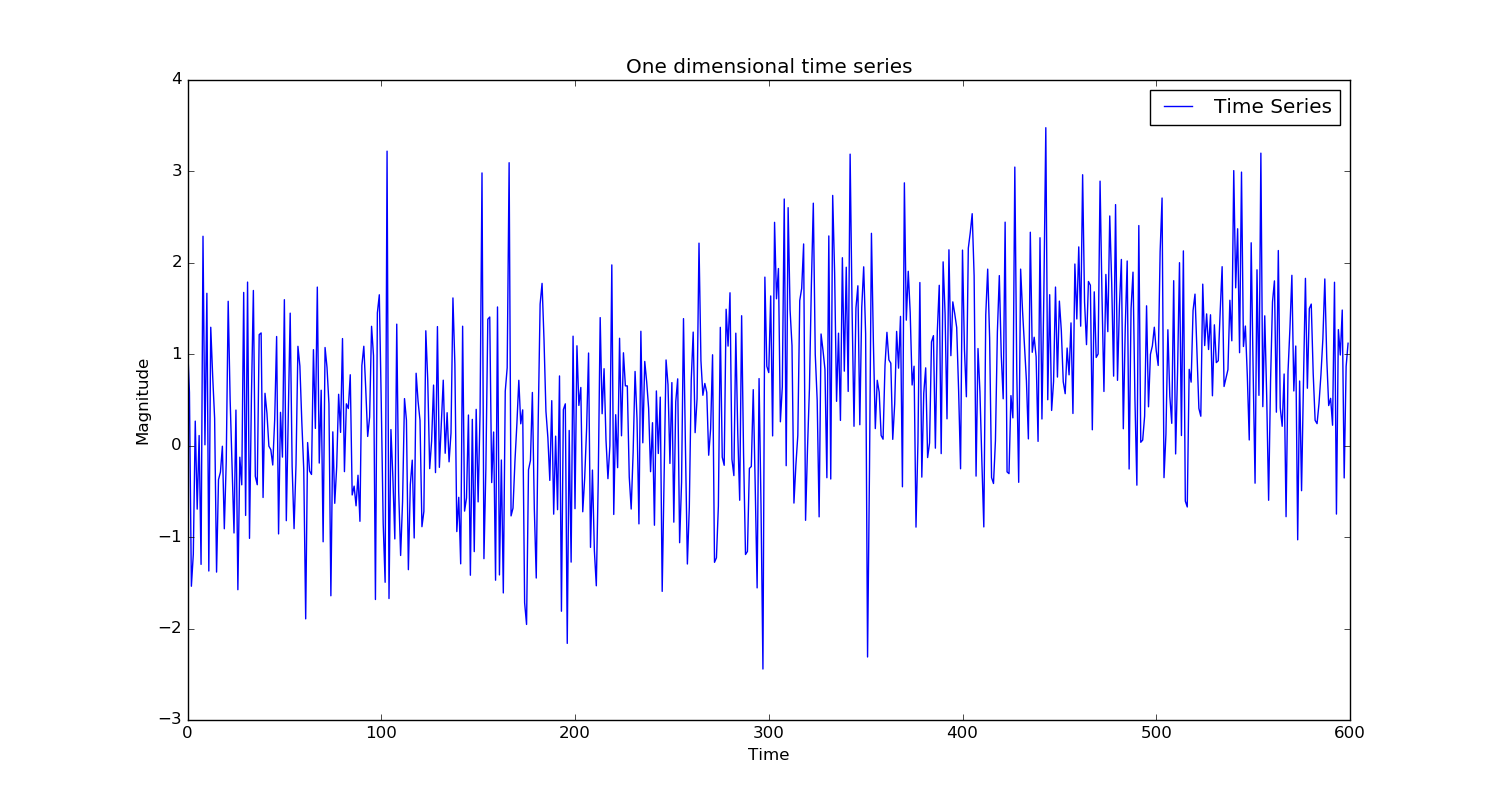
\includegraphics[width=1\textwidth]{images/1d_offline/ts}
  \caption{One dimensional time series.\label{fig:1d_ts}}
\end{figure}

\begin{figure}[ht!]
  \centering
  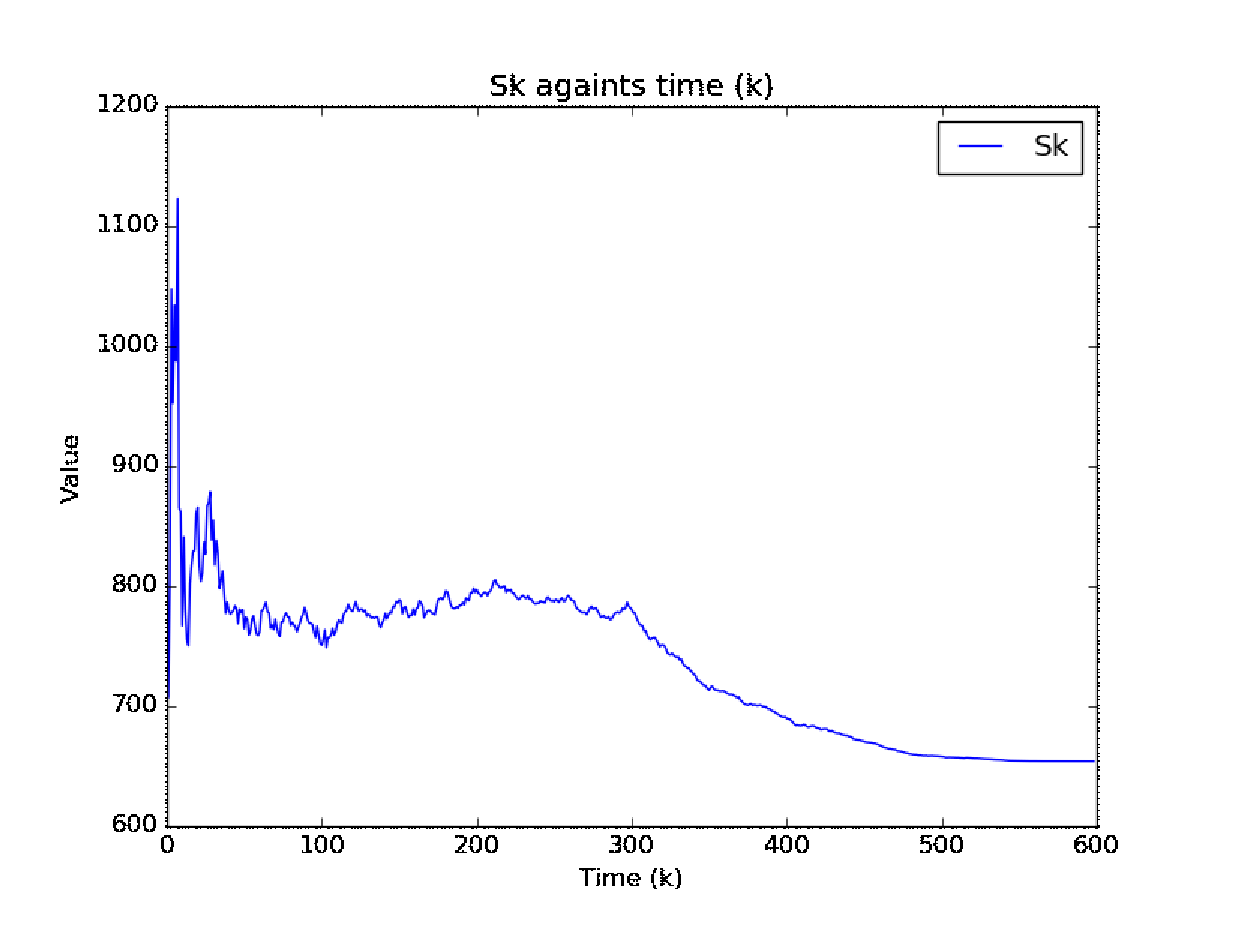
\includegraphics[width=0.75\textwidth]{images/1d_offline/sk}
  \caption{SK values for one dimensional offline detection problem.\label{fig:1d_sk}}
\end{figure}

\begin{figure}[ht!]
  \centering
  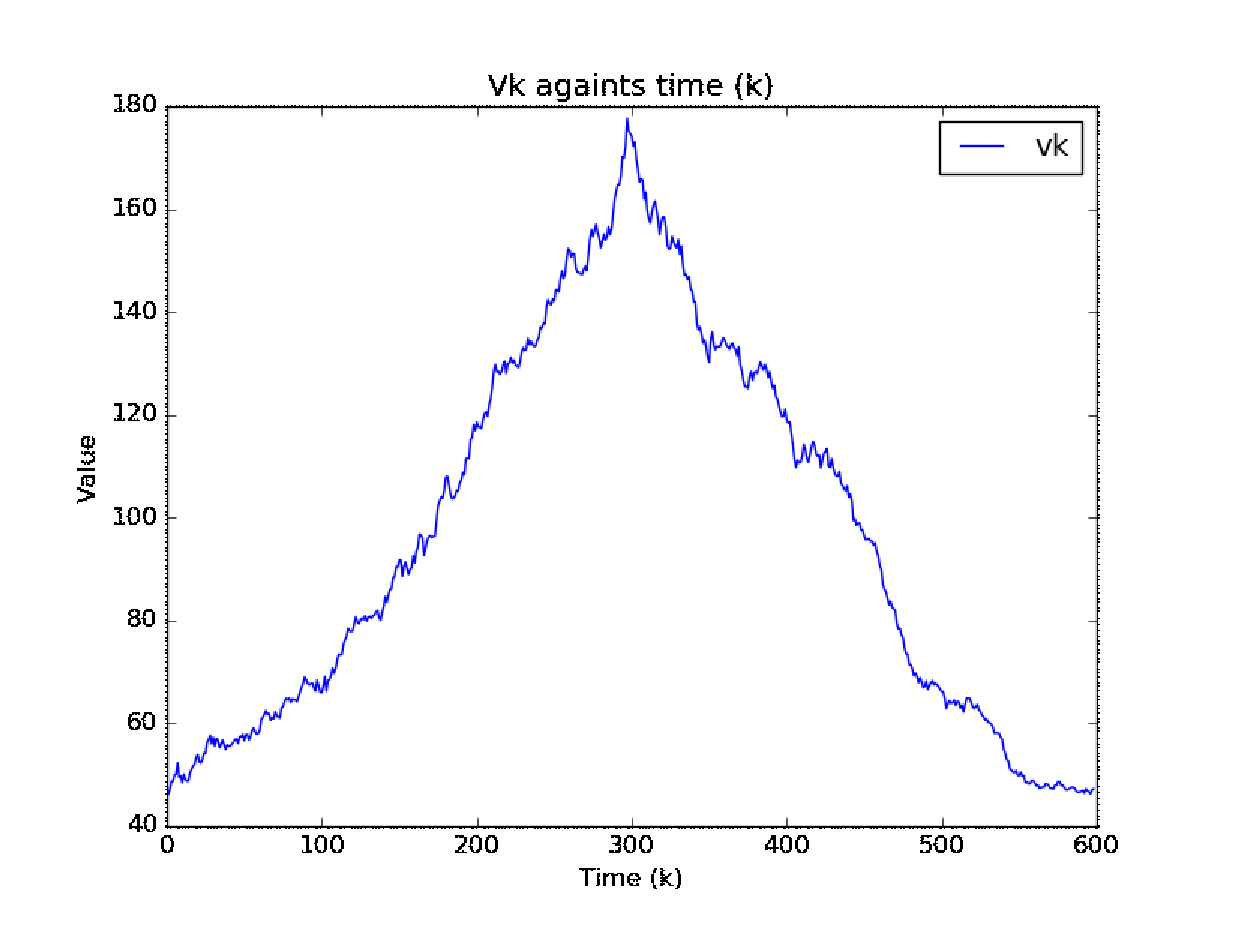
\includegraphics[width=0.75\textwidth]{images/1d_offline/vk}
  \caption{VK values for one dimensional offline detection problem.\label{fig:1d_vk}}
\end{figure}


\subsubsection{Multivariate Time series}

Multivariate model is similar to the above Univariate model except that each and every observation is m-dimensional.
Let $x_{1}, x_{2}, \ldots , x_{n}$ be a sequence of independent $m$-dimensional normal random vectors with parameters $(\mu_{1}, \Sigma_{1}), (\mu_{2}, \Sigma_{2}), \ldots, (\mu_{n}, \Sigma_{n})$, respectively.
Assume $\Sigma_{1} = \Sigma_{2} = \cdots = \Sigma_{n} = \Sigma $.
The null hypothesis is given by 
\begin{align}
H_{0} : \mu_{1} = \mu_{2} = \cdots = \mu_{n} = \mu (\mathrm{unknown})
\end{align}

If we assume that there is a change at point $k$ in the paramters governing the observation, then the hypothesis (alternate hypothesis) is given by

\begin{align}
H_{1} : \mu_{1} = \cdots = \mu_{k} \ne \mu_{k+1} = \mu_{n}
\end{align}
Where k represents the position of the single change point. (Refer 3.1 of~\cite{birkhauser_pscpa}).

This can be solved by following the steps described in section 3.1.1 of~\cite{birkhauser_pscpa}.  As in the case of univariate model, finding the likelihood directly is computationally intractable as $2\pi$ and $e$ has negative powers that can go pretty large and hence the likelihood will always become 1.

\subsubsection{Experiments --- Multivariate change point detection}
We did Several experiments by varying the number of dimension and also the total number of samples.  So far, in all variations, we are able to identify the change point pretty accurately using the offline detection method described above.  The plots below are for dimension = 6 and number of samples = 600 with change point at 300.

\begin{figure}[ht!]
  \centering
  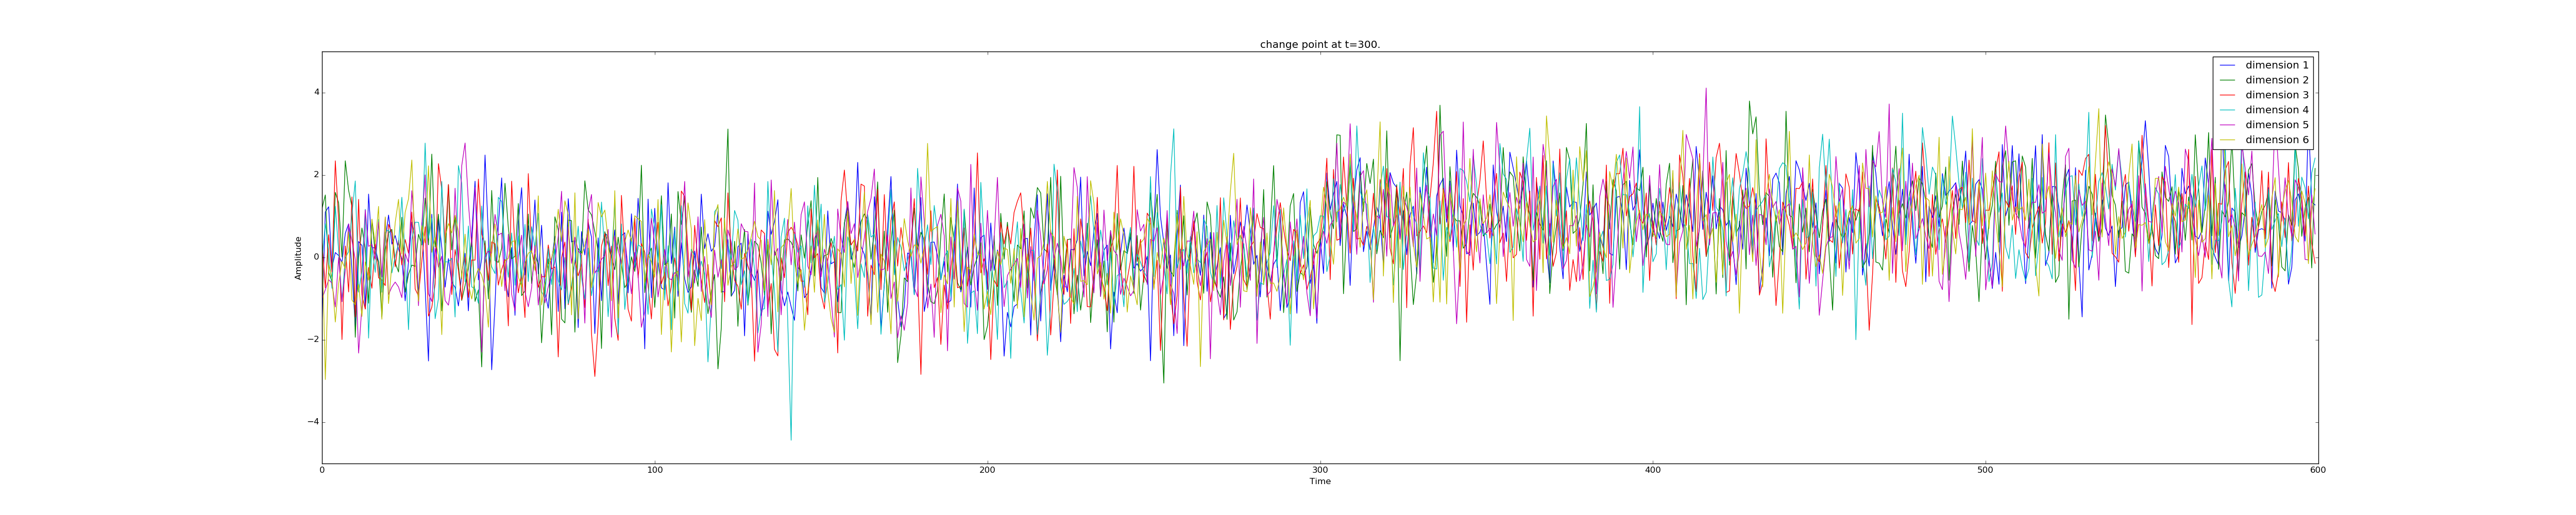
\includegraphics[width=1\textwidth]{images/rd_offline/ts}
  \caption{Multi dimensional time series.\label{fig:rd_ts}}
\end{figure}

\begin{figure}[ht!]
  \centering
  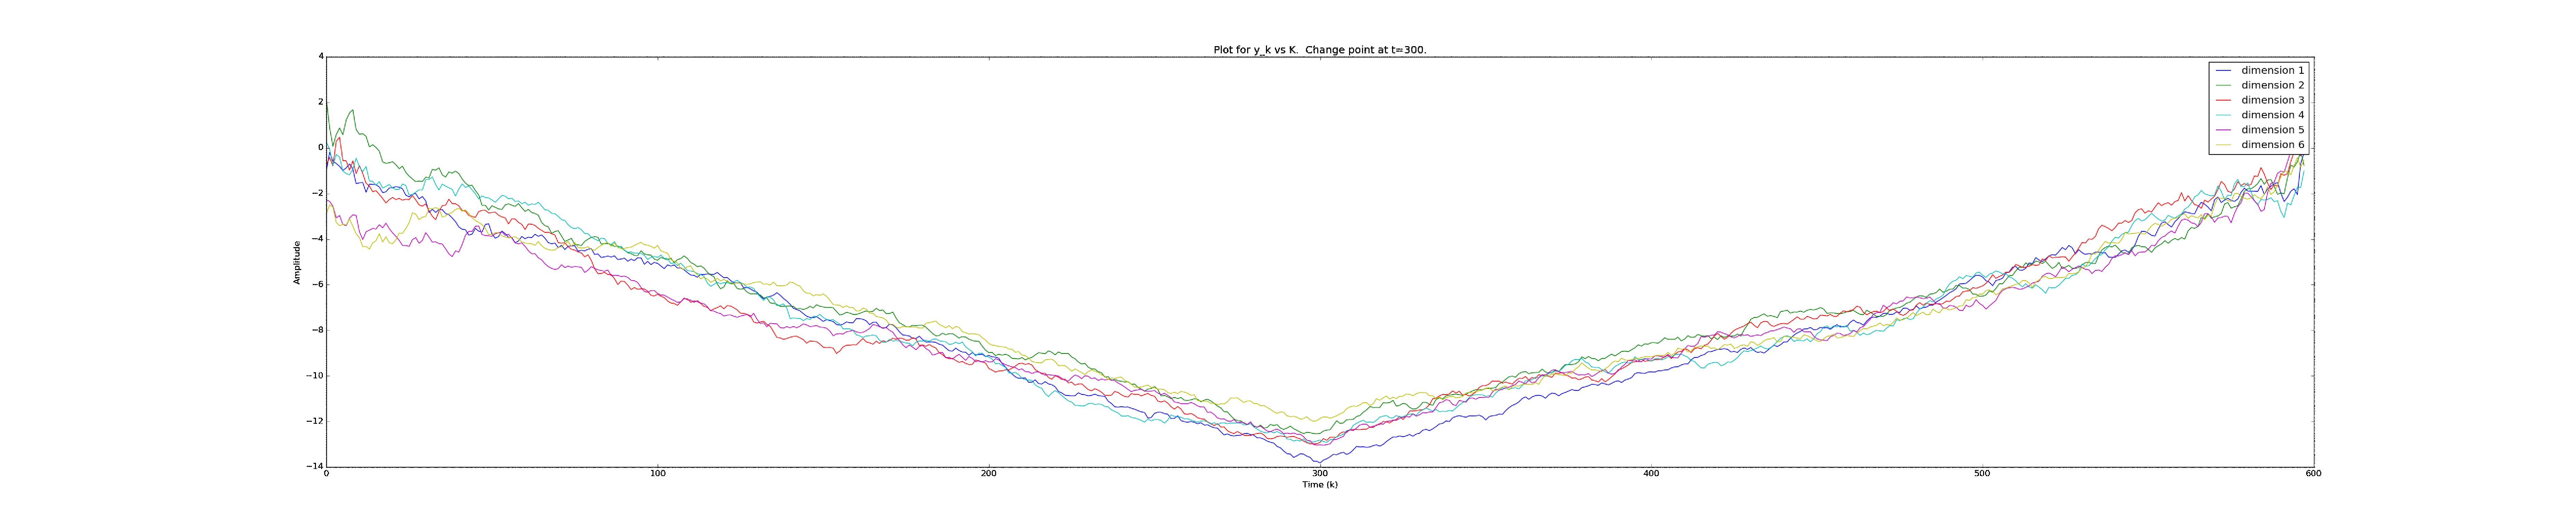
\includegraphics[width=1\textwidth]{images/rd_offline/y_k}
  \caption{Value of y\_k with respect to various k.\label{fig:rd_y_k}}
\end{figure}

\begin{figure}[ht!]
  \centering
  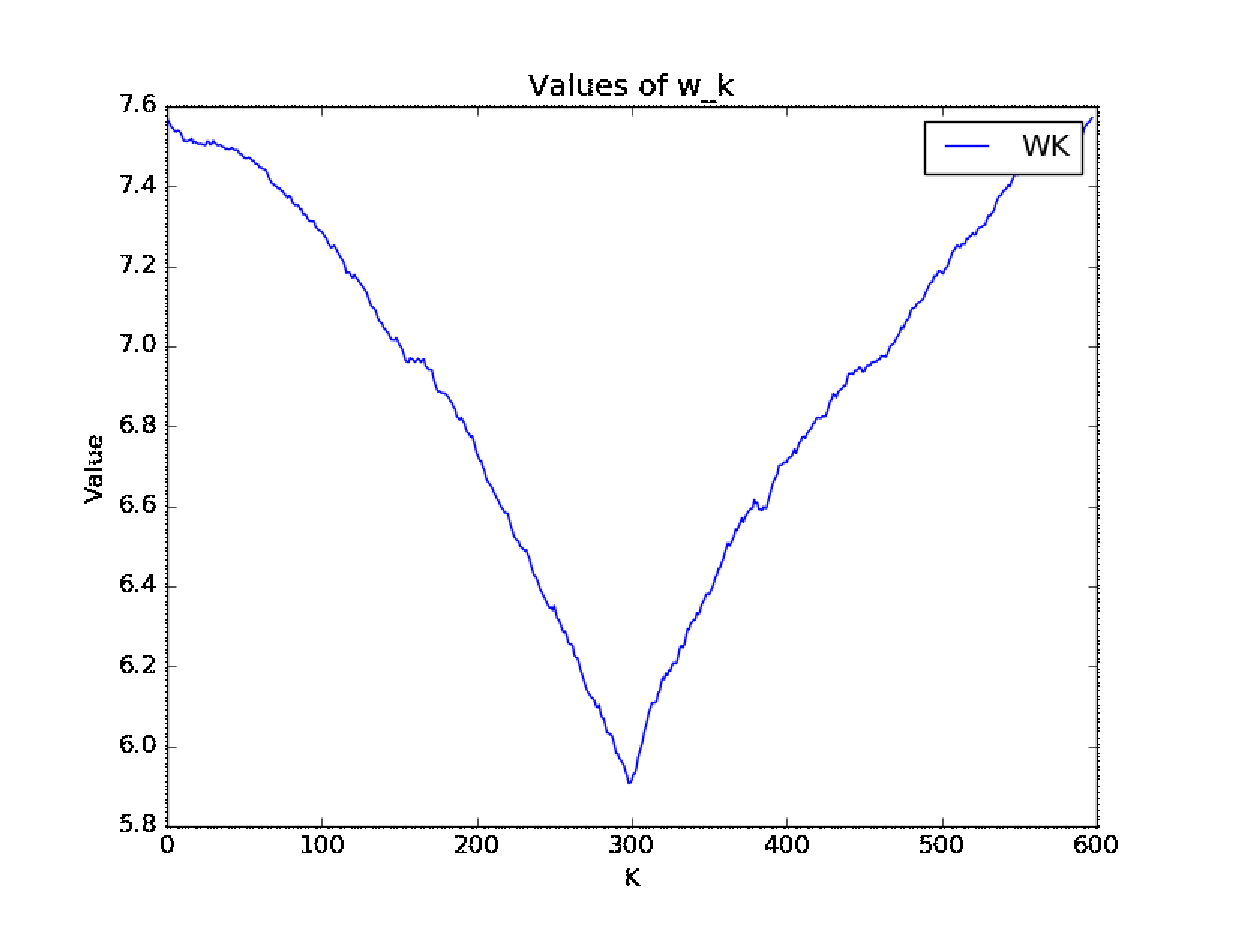
\includegraphics[width=0.75\textwidth]{images/rd_offline/w_k}
  \caption{Value of w\_k with respect to various k.\label{fig:rd_w_k}}
\end{figure}

\begin{figure}[ht!]
  \centering
  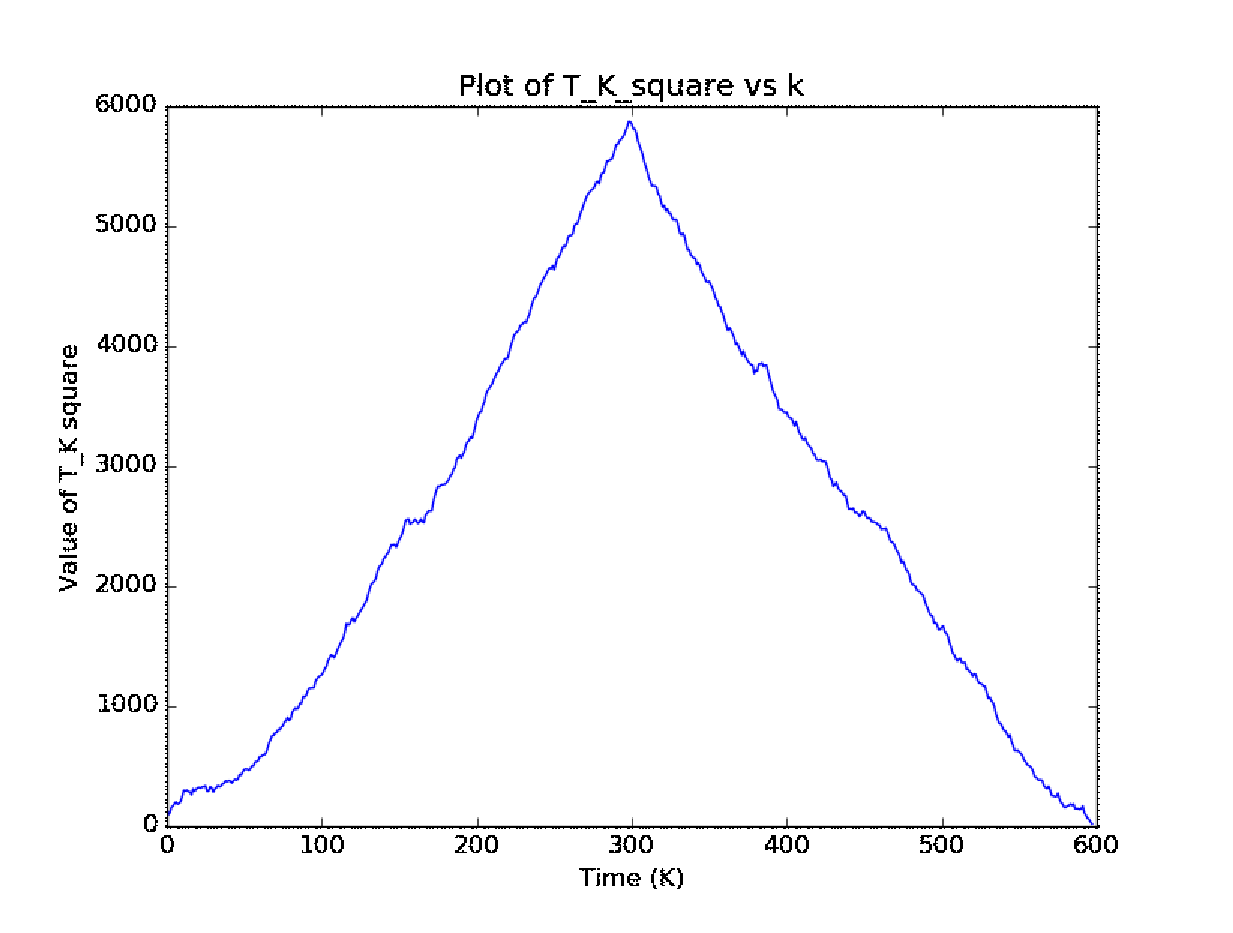
\includegraphics[width=0.75\textwidth]{images/rd_offline/tk_sq}
  \caption{Value of the test stastic $ T_{k}^{2} $ with respect to various k.\label{fig:rd_tk_sq}}
\end{figure}


\subsection{Online Change point detection}
Online detection of change point is slightly difficult than offline detection. We have a series of observation defined by $x_{1}, x_{2}, \ldots, x_{n} $.  Each observation denoted by $x_{i}$ is assumed to be made of N samples.

We start by defining a sufficient stastic as:
\begin{align}
  s_{i} = \ln{\frac{p\theta_{1}(y_{i})}{p\theta_{0}(y_{i})}}
\end{align}

We also define a decision rule d given by
\begin{align}
  d = \begin{cases}
    0 & if S_{1}^{N} < h; H_{0} \text{~is chosen}\\
    1 & if S_{1}^{N} \ge h; H_{1} \text{~is chosen}\\
      \end{cases}
\end{align}

Where h is a threshold chosen by the user.  $S_{1}^{N}$ is called as the decision function.

We also have a stopping rule which is defined by 
\begin{align}
  t_{a} = N.\min{K : d_{K} = 1}
\end{align}
Where d is the decision taken with the aid of the decision function defined above.  This method of finding the stopping rule and alarm time is as given in\cite{basseville_nikiforov}

\subsubsection{Experiments --- Online change point detection}

We run experiments using grid search with various values of h and kappa.  In this particular experiment, we used values ranging from 1.5 to 5.5 with step size 0.25 for h and 0.5 to 4 with step size of 0.25 for kappa.  We then proceed to find all the values of the stopping rule and also the alarm time for h and kappa combination.  The time series, the plots for alarm time and stopping rule are plotted below.

\begin{figure}[ht!]
  \centering
  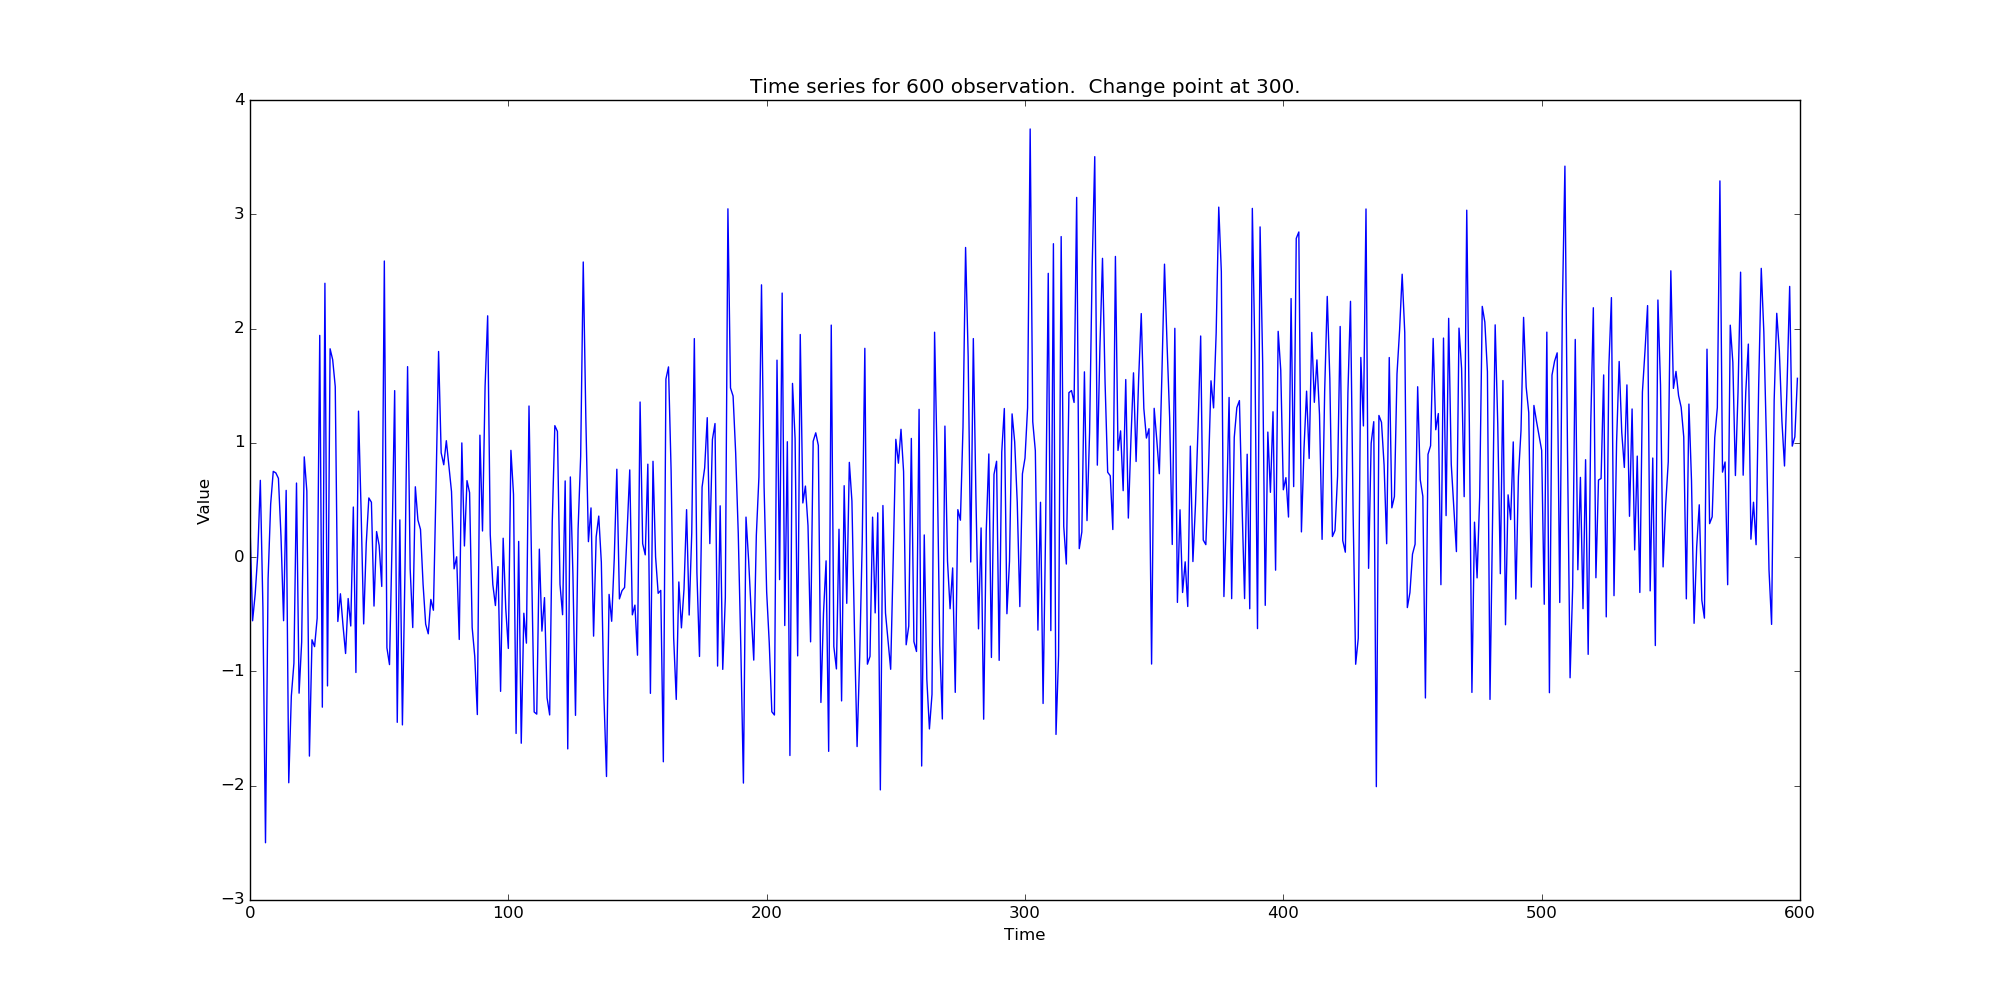
\includegraphics[width=1\textwidth]{images/1d_online/ts}
  \caption{One dimensional time series for online detection.\label{fig:1d_o_ts}}
\end{figure}

\begin{figure}[ht!]
  \centering
  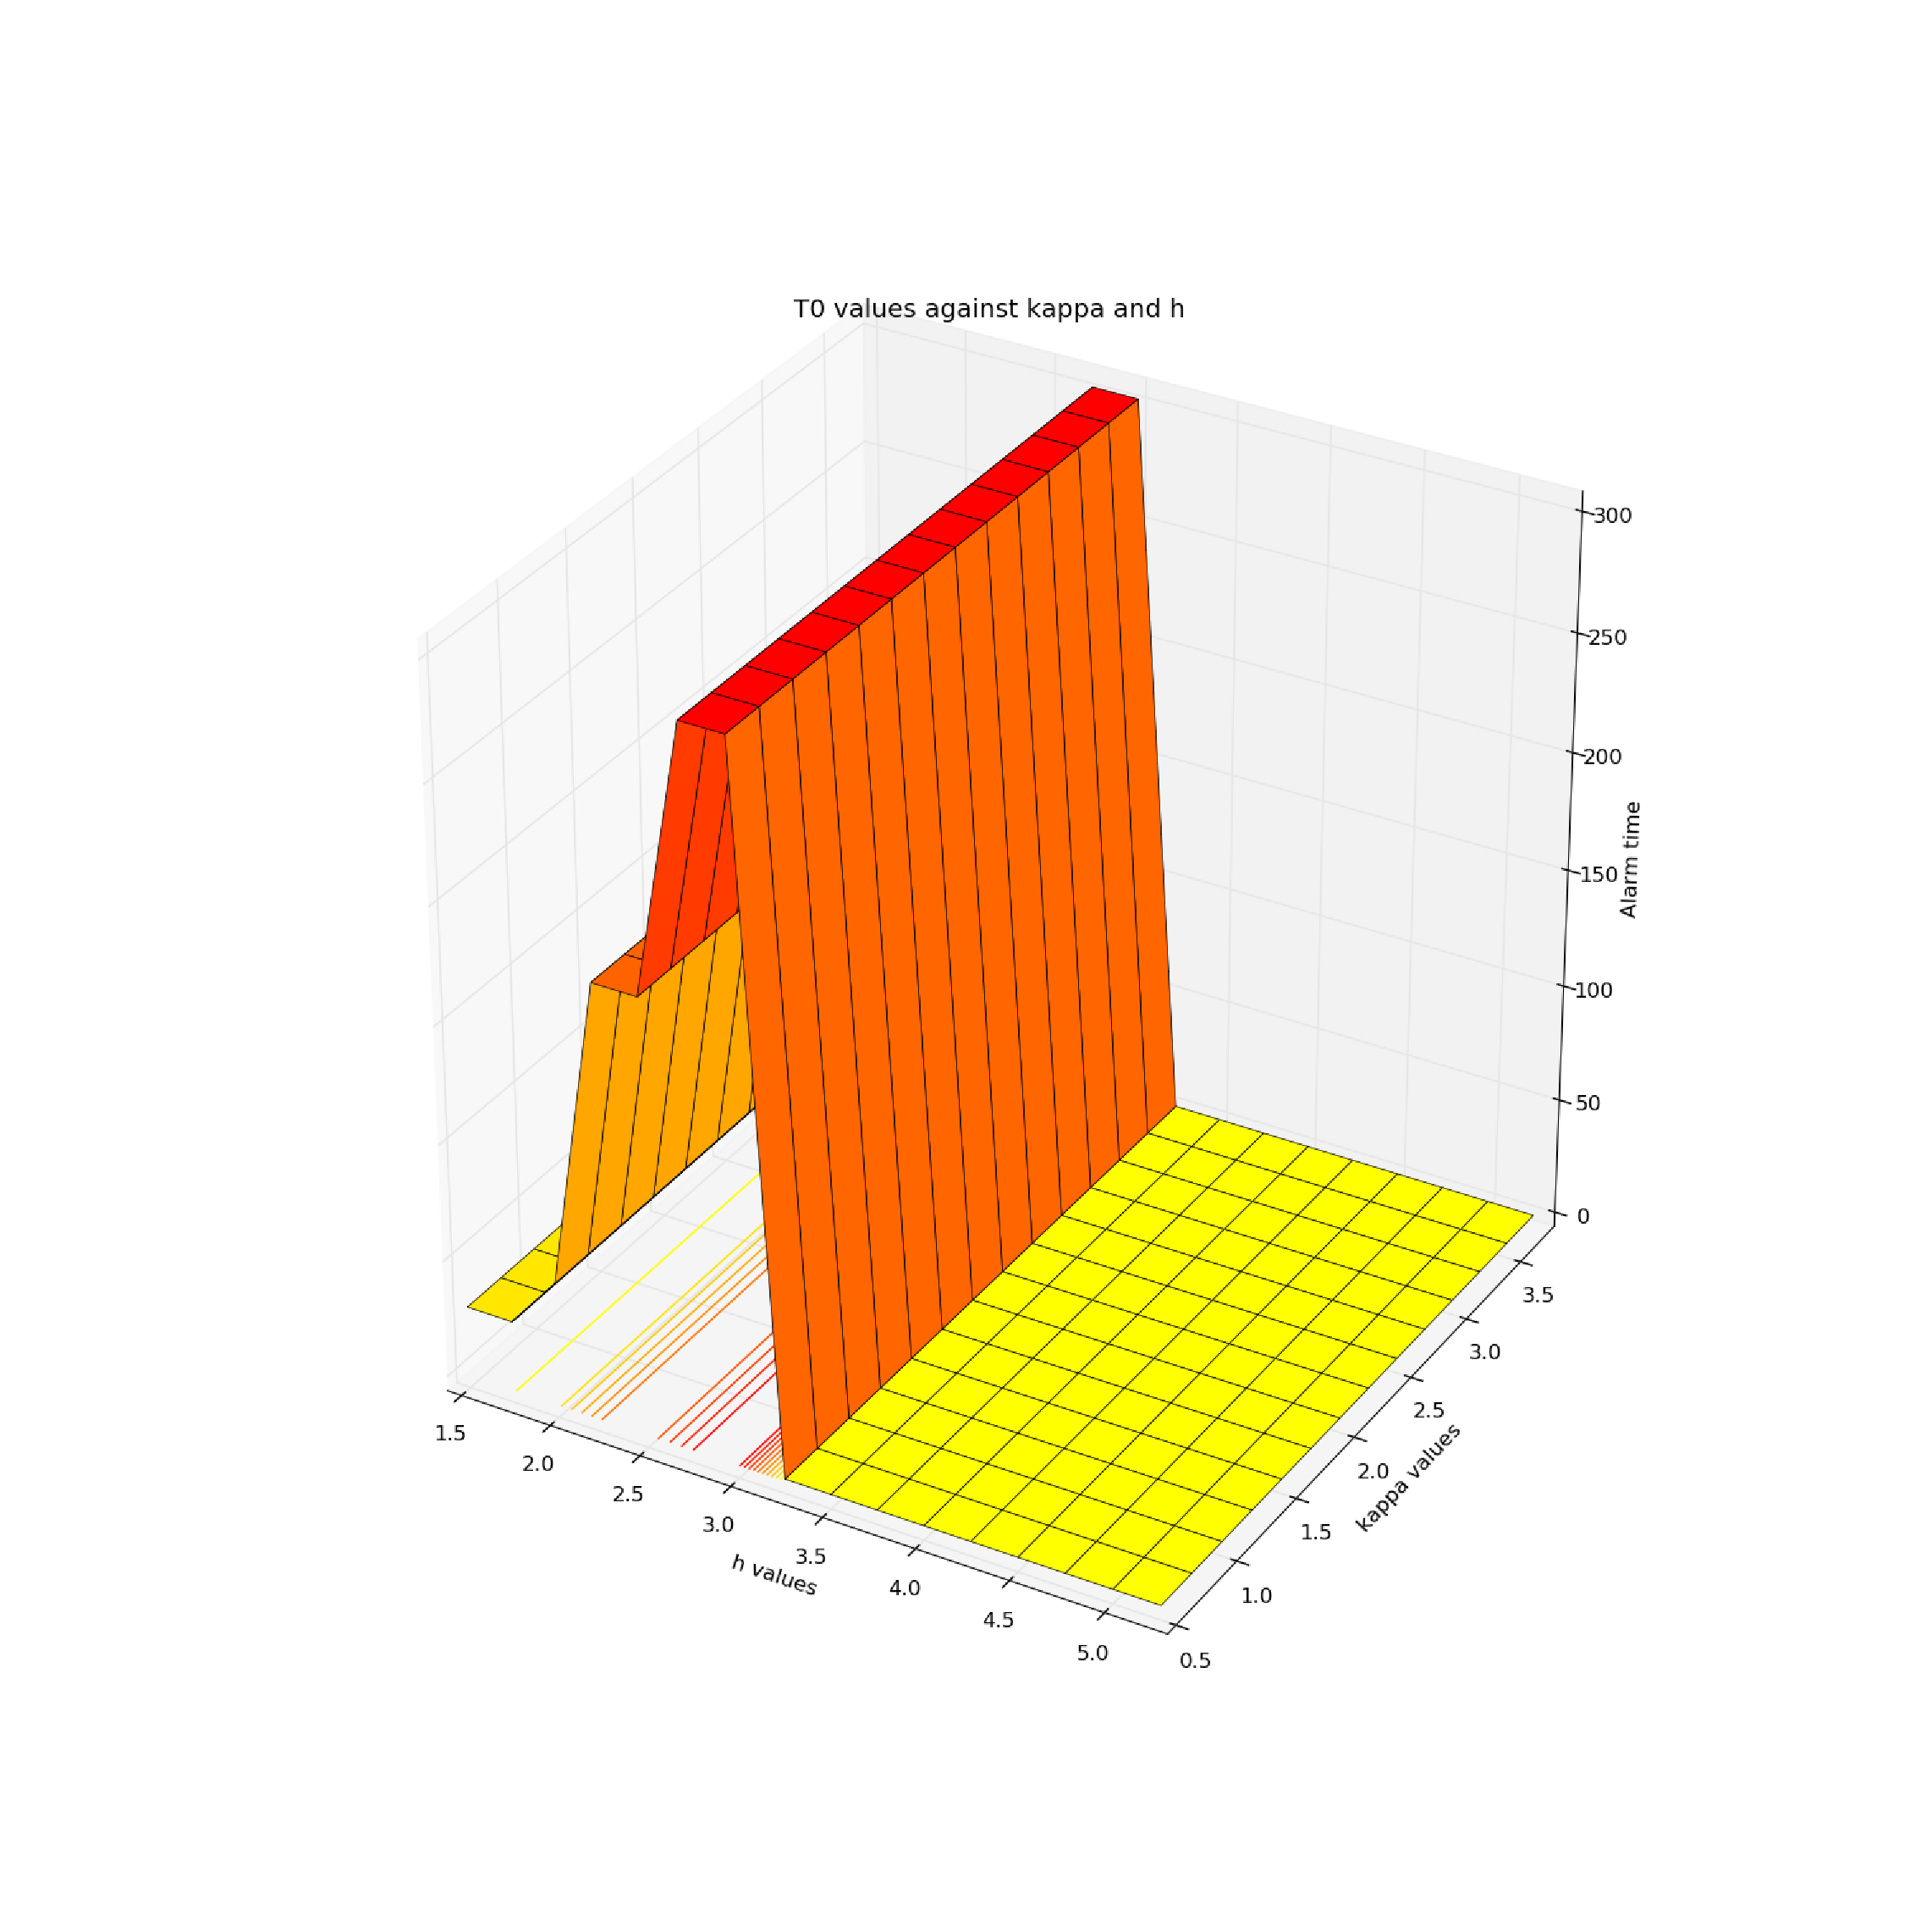
\includegraphics[width=0.75\textwidth]{images/1d_online/time}
  \caption{Stopping rule for various values of h and kappa.\label{fig:1d_o_time}}
\end{figure}

\begin{figure}[ht!]
  \centering
  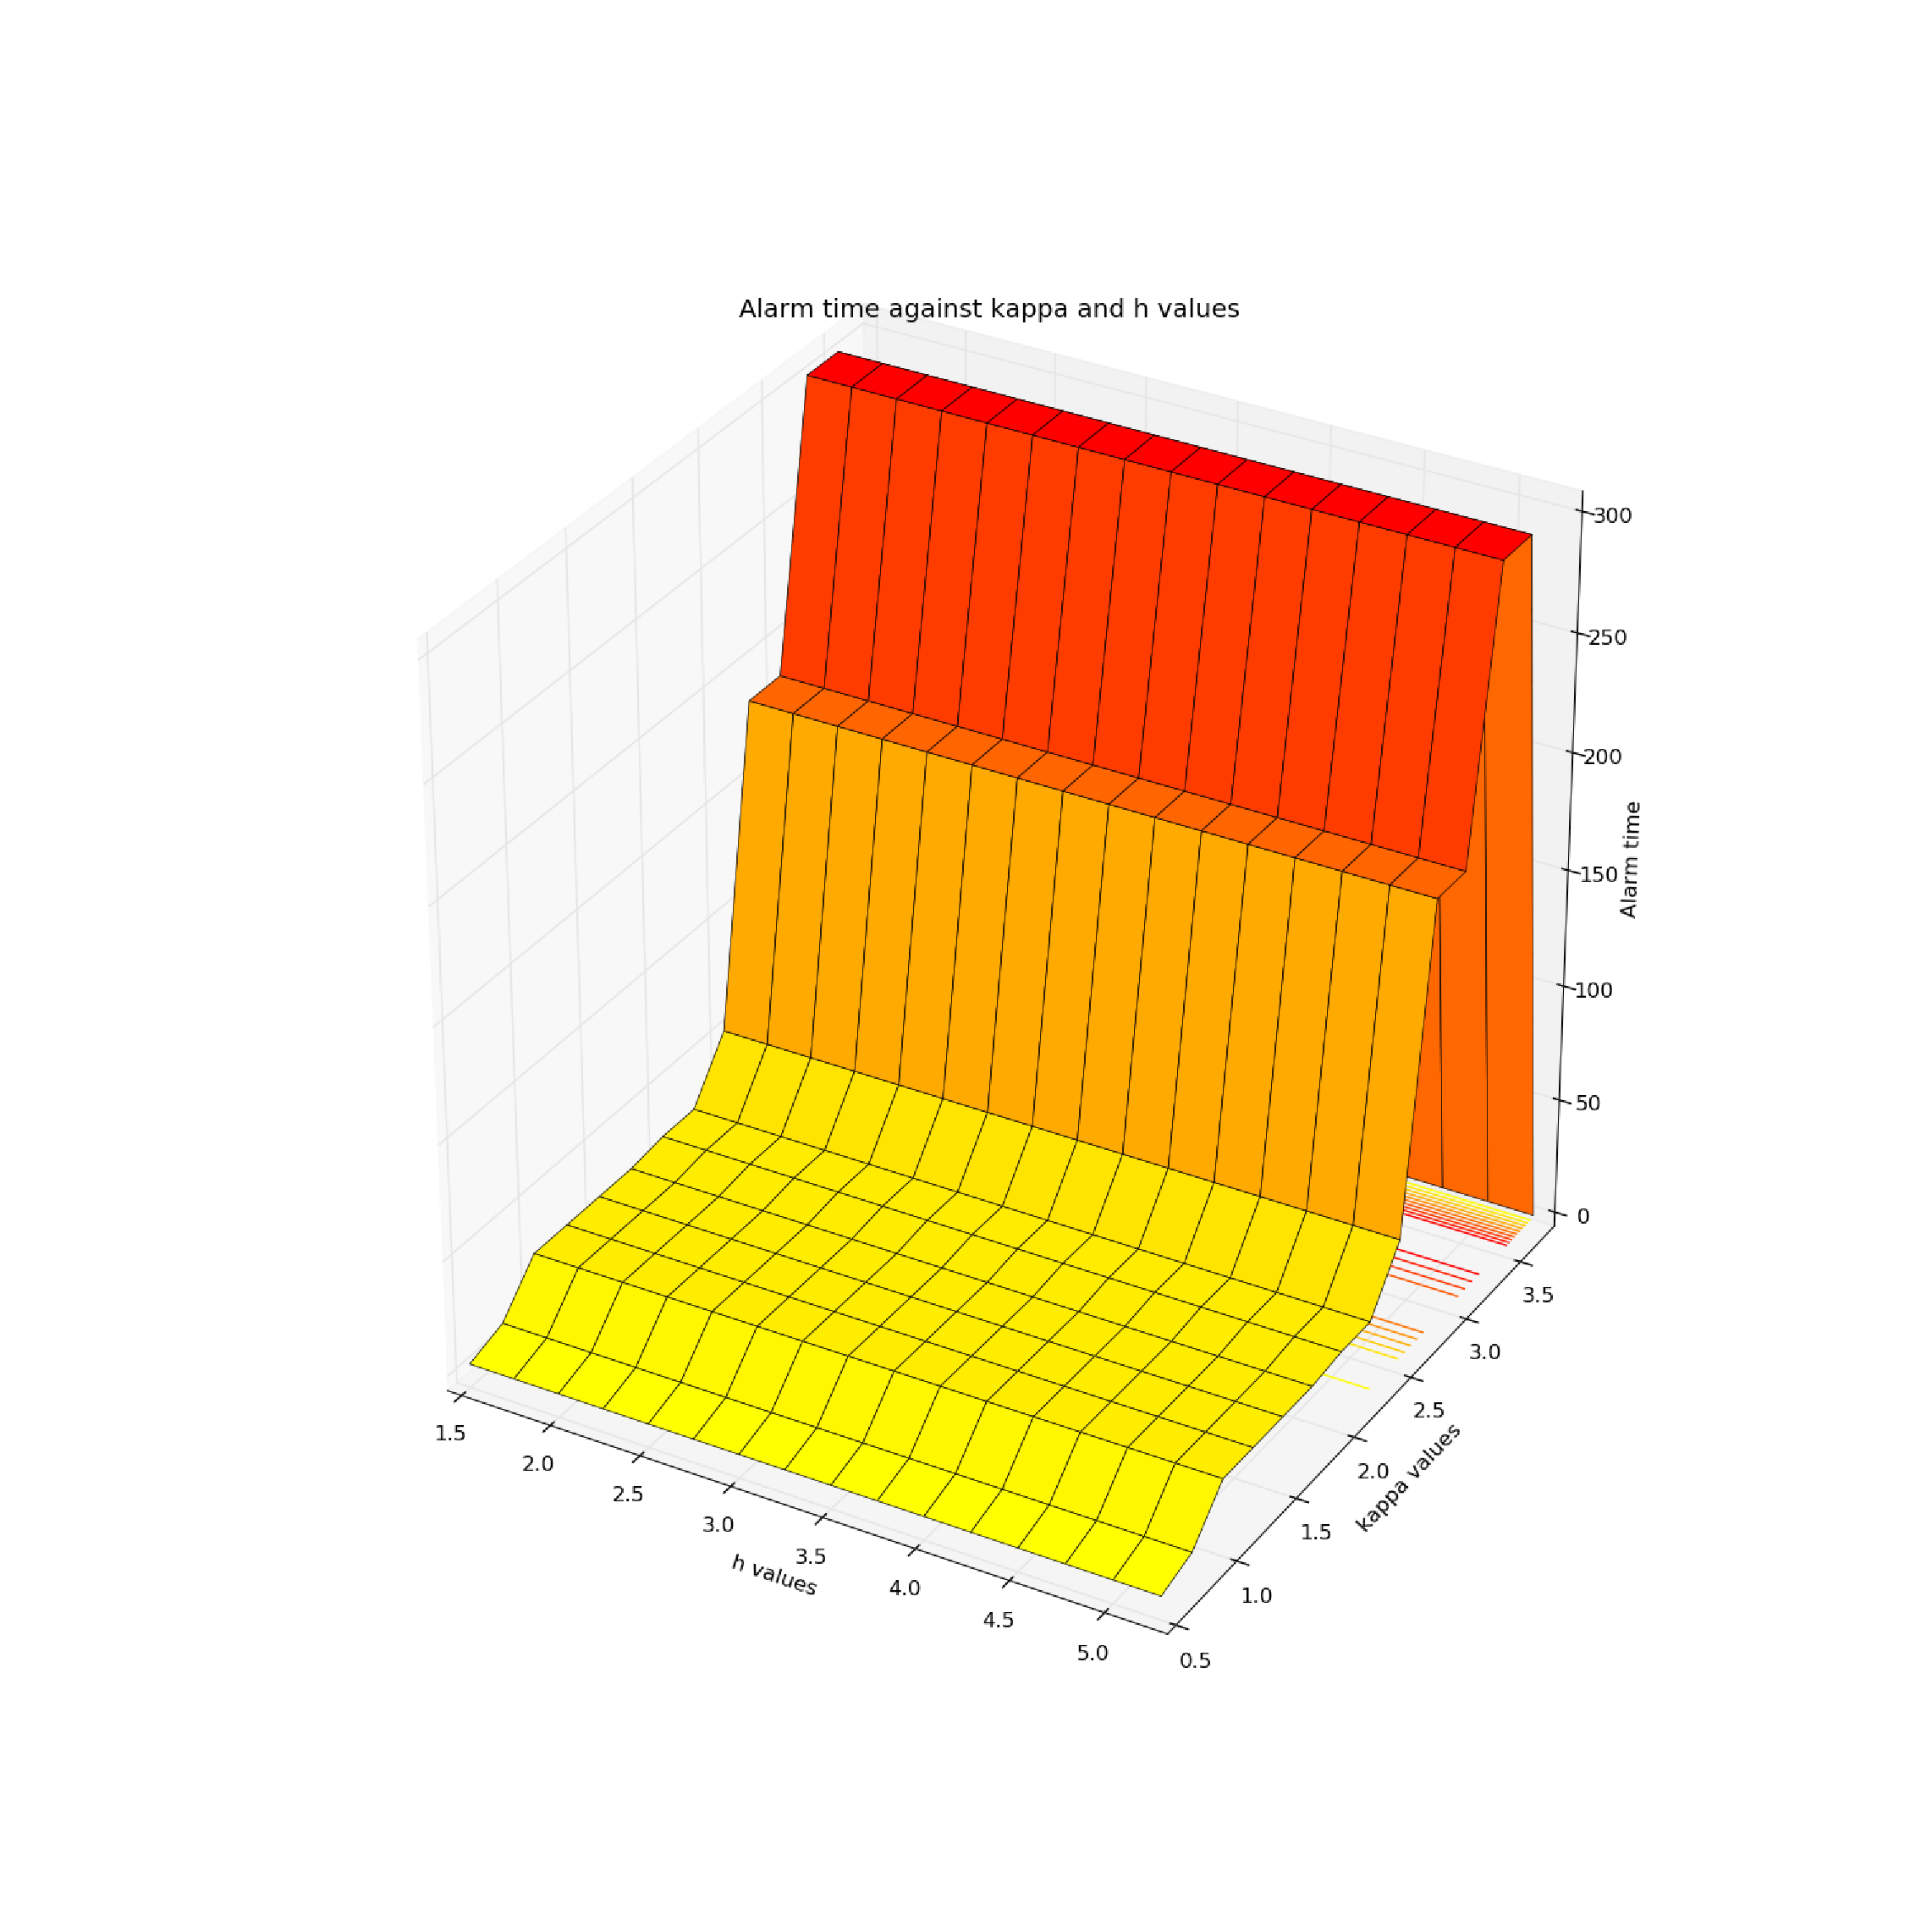
\includegraphics[width=0.75\textwidth]{images/1d_online/alarm}
  \caption{Alarm time for values of h and kappa.\label{fig:1d_o_alarm}}
\end{figure}

\section{Spectral Density}
\subsection{Auto CoVariance Function}
\subsection{Auto Corelation Function}
\subsection{Peridogram}
\subsection{Change points using spectral density}

\bibliographystyle{plain}
\bibliography{references}
\end{document}
